\section*{Exercice 147 -- PFS}
\setcounter{exo}{0}
%E3A MP 2009

%\subsection*{Asservissement de position du palier magnétique actif}
On s'intéresse à un système d'enroulage de papier.

La figure suivante représente une bobine fille et des rouleaux porteurs.  Un mandrin sert de support à la bobine fille. Sur ce mandrin, vient s'enrouler du papier kraft. 


\begin{center}
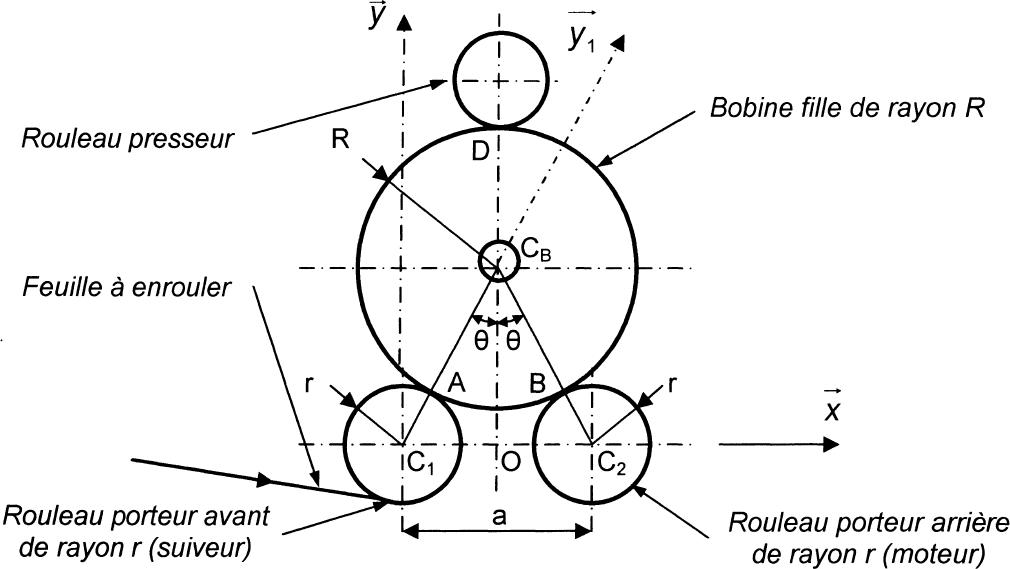
\includegraphics[width=\linewidth]{988_01}%
\end{center}

\subsubsection*{Notations}
\begin{itemize}
\item $C_B$ : centre de la bobine fille de rayon $R$.
\item $C_1$ et $C_2$ : centres respectifs des rouleaux porteurs avants et arrières de rayon $r$.
%\item $C_2$ : centre du rouleau porteur arrière de rayon $r$.
\item $A$ et $B$ : points de contact respectifs entre les rouleaux porteurs avants et arrières et la bobine fille.
%\item $B$ : point de contact entre le rouleau porteur arrière et la bobine fille.
\item $O$ : point milieu entre $C_1$ et $C_2$.
\item $a$ : entraxe entre les deux rouleaux porteurs.
\item $R$ : rayon de la bobine fille (\SI{900}{mm} maxi).
\item $L$ : longueur de la bobine fille (\SI{5080}{mm} maxi).
\item $R_M = \SI{100}{mm}$ : rayon du mandrin.
\item $F$ : force appliquée par le rouleau presseur sur la bobine fille. 
\item $T$ : tension de la feuille exprimée au point $A$.
\item $P_B$ : poids de la bobine;
\item $R_A$ et $R_B$ : efforts respectifs des rouleaux porteurs avants et arrières sur la bobine fille.  
\item $C_M$ : couple d’entraînement appliqué au rouleau arrière (moteur).
\item $r$ : rayon du rouleau porteur arrière et du rouleau porteur avant. 
\item $f=\tan\varphi = 0,3$ : coefficient de frottement du rouleau porteur / papier.  
\item $\rho_v = \SI{800}{kg.m^{-3}}$ : masse volumique du papier.
\end{itemize}

\subsubsection*{Hypothèses}

L'élasticité longitudinale de la feuille de papier est supposée négligeable.
Les inerties des deux rouleaux porteurs autour de leur axe sont négligeables devant la masse de la bobine. La bobine fille tourne à vitesse constate. L'étude est faite en se plaçant aux conditions limites d'adhérence.
On souhaite dans un premier temps, établir la loi de variation temporelle de l'effort presseur nécessaire à l'obtention d'une densité constante.


\subparagraph{}
\textit{En considérant que l'empilement des feuilles sur la bobine est homogène, donner l'expression littérale du poids de la bobine. Tracer l'allure de la courbe du poids de la bobine en fonction de son rayon : $P_B = f(R)$.}
\ifprof
\begin{corrige} En considérant le poids de la bobine de papier seul, on a directement 
$P_B (R)= \rho_v L \pi \left(R^2 - R_M^2 \right) g$
\end{corrige}
\else
\fi

\subparagraph{}
\textit{Faire l'application numérique pour une bobine fille de taille maximale.}
\ifprof
\begin{corrige}
\end{corrige}
\else
\fi

\subparagraph{}
\textit{À partir de la figure précédente en isolant la bobine fille, déterminer une relation vectorielle liant l'effort presseur 
$\vect{F(t)}$, $\vect{R_A}$, $\vect{R_B}$, $\vect{P_B}$ et $\vect{T}$. }
\ifprof
\begin{corrige}
On isole la bobine.

BAME : poids de la bobine $\vect{P_B}$, efforts presseurs des rouleaux en $A$ et en $B$, tension $\vect{T}$ de la feuille en $A$, effort du rouleau presseur.

TRS : $\vect{F(t)} + \vect{R_A} + \vect{R_B} + \vect{P_B} + \vect{T} = \vect{0}$
\end{corrige}
\else
\fi


\subparagraph{}
\textit{En isolant la bobine fille, représenter sur le document suivant les actions mécaniques au point $A$ et au point $B$.}
\ifprof
\begin{corrige}
Les efforts des rouleaux porteurs se décomposent en un effort tangentiel et un effort normal, orienté vers $C_B$.


\begin{center}
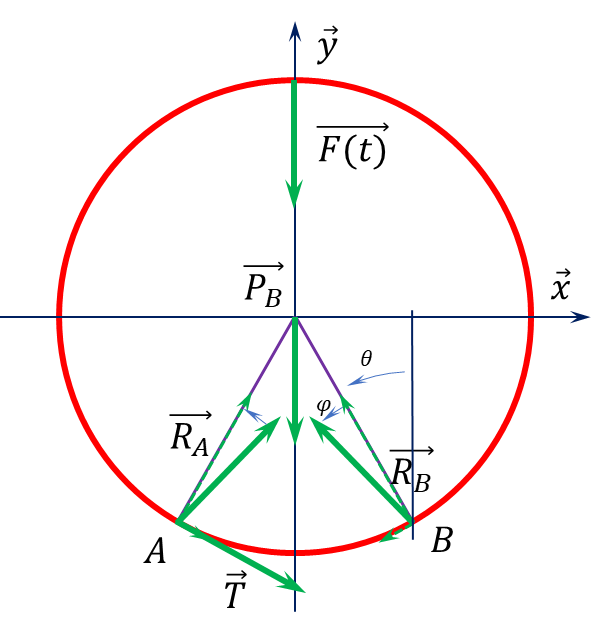
\includegraphics[width=.35\linewidth]{988_03}%
\end{center}

\end{corrige}
\else
\begin{center}
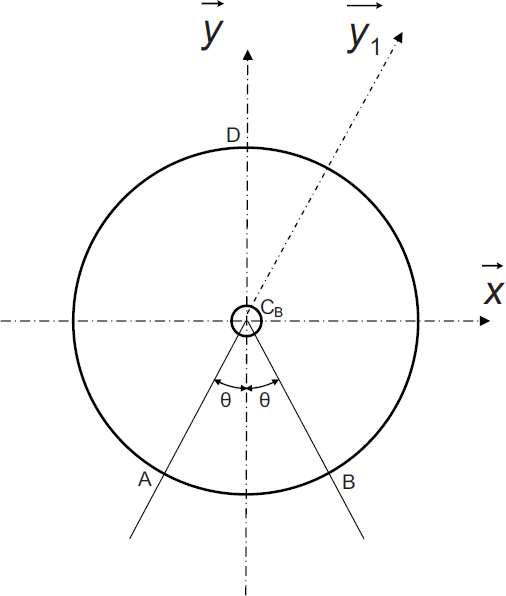
\includegraphics[width=\linewidth]{988_02}%
\end{center}
\fi



\subparagraph{}
\textit{En utilisant l'hypothèse sur l'inertie des rouleaux, montrer que l'on peut écrire le couple moteur du rouleau porteur arrière sous la forme $C_M=rT_B$, avec $T_B$ composante tangentielle de l'action $R_B$.}
\ifprof
\begin{corrige}
On isole le rouleau porteur arrière.

BAME : action de la bobine fille en $B$, action de la pesanteur sur la bobine fille en $C_2$, couple moteur en $C_2$. 

Si on néglige l'inertie de la bobine arrière, on peut appliquer le théorème du moment statique en $C_2$ en projection sur $\vect{z}$ :
\begin{itemize}
\item $\vectm{C_2}{\text{fille}}{\text{porteur ar}} = \vect{C_2 B} \wedge \vect{R_B} = \pm r T_B$; 
\item $\vectm{C_2}{\text{pes}}{\text{porteur ar}} = \vect{0}$; 
\item $C_m$.
\end{itemize}
Au final $C_m = \pm r T_B$.

\end{corrige}
\else
\fi


\subparagraph{}
\textit{Déterminer l'expression de la tension de la feuille $T$.}
\ifprof
\begin{corrige}
On projette l'expression de la question 4 sur $\vect{x}$ et on a 

$R_A \sin \left(\theta+\varphi\right) - R_B\sin \left(\theta+\varphi\right) + T \cos\theta = 0$

soit
$T =\left(R_B  -R_A\right) \dfrac{\sin \left(\theta+\varphi\right)}{\cos\theta } $
\end{corrige}
\else
\fi


\subparagraph{}
\textit{En projetant la relation vectorielle de la question 4 sur $\vect{y}$, donner l'expression de l'effort presseur $F$ en fonction de $T$, $R_A$, $R_B$ $P_B$, $\varphi$ et $\theta$.}
\ifprof
\begin{corrige}
On projette l'expression de la question 4 sur $\vect{y}$ et on a 

\noindent $R_A \cos \left(\theta+\varphi\right) - R_B\cos \left(\theta+\varphi\right) - T \sin\theta -F(t)-P= 0$ 

soit

$F(t)=R_A \cos \left(\theta+\varphi\right) - R_B\cos \left(\theta+\varphi\right) - T \sin\theta -P$.

En utilisant le résultat de la question précédente, on a : 

$F(t)=R_A \cos \left(\theta+\varphi\right) - R_B\cos \left(\theta+\varphi\right) - \left(R_B  -R_A\right) \dfrac{\sin \left(\theta+\varphi\right)}{\cos\theta } \sin\theta -P$.

et


$F(t)=R_A \cos \left(\theta+\varphi\right) - R_B\cos \left(\theta+\varphi\right) - \left(R_B  -R_A\right)\sin \left(\theta+\varphi\right)  \tan \theta -P$.

\end{corrige}
\else
\fi


\begin{enumerate}
\item $P_B = \rho_v \pi \left(R^2 - R_M^2 \right)Lg$.
\item $P_B = \SI{101764}{N}$.
\item $\vect{F}+\vect{R_A}+\vect{R_B}+\vect{P_B}+\vect{T}=\vect{0}$.
\item ...
\item $C_m = rR_B$.
\item $T =\left(R_B  -R_A\right) \dfrac{\sin \left(\theta+\varphi\right)}{\cos\theta } $.
%$T = \dfrac{R_B \sin \left( \varphi+ \theta \right)- R_A \sin\theta }{\cos \theta }$ 
\item $F(t)=R_A \cos \left(\theta+\varphi\right) - R_B\cos \left(\theta+\varphi\right) - \left(R_B  -R_A\right)\sin \left(\theta+\varphi\right)  \tan \theta -P$.
\end{enumerate}